\chapter{Design}
\label{sec:Design}

This chapter of the report documents the design process for the laparoscope. From determining the design requirement, to concept design generation, and detail design of the laparoscope.

\section{Design Requirements for Laparoscope}

This section documents the list of requirements that need to be determined to be able to design a functional laparoscope. These requirements are all listed in the tables below, as well as depicted  in the diagrams below. 

\subsection{Stakeholder Analysis}

The stakeholder analysis is shown in Table \ref{tab:stakeholders} below:

\begin{longtable}{|p{0.10\textwidth}|p{0.10\textwidth}|p{0.121\textwidth}|p{0.18\textwidth}|p{0.12\textwidth}|p{0.18\textwidth}|}

    \caption{Stakeholder analysis}              % ← Moved to top
    \label{tab:stakeholders}\\
% ---- FIRST PAGE HEADER ----
\hline
\textbf{Stake-holder ID} & 
\textbf{Stake-holder} & 
\textbf{Class-ification} & 
\textbf{Description} & 
\textbf{Life Cycle Stages} & 
\textbf{Key Interest/Needs} \\
\hline
\endfirsthead

% ---- SUBSEQUENT PAGE HEADER ----
\hline
\textbf{Stake-holder ID} & 
\textbf{Stake-holder} & 
\textbf{Class-ification} & 
\textbf{Description} & 
\textbf{Life Cycle Stages} & 
\textbf{Key Interest/Needs} \\
\hline
\endhead

% ---- FOOTER ALL PAGES EXCEPT LAST ----
\hline
\multicolumn{6}{r|}{\textit{Continued on next page...}} \\
\hline
\endfoot

% ---- LAST PAGE FOOTER ----
\endlastfoot

% ---- SH_01 ----
SH\_01 & 
Dr Diayar & 
Indirect & 
The doctor that recommend the development of the system & 
Concept & 
The functional development of the system \\
\hline

% ---- SH_02 ----
SH\_02 & 
Prof Schreve & 
Secon-dary & 
Supervisor of the project & 
All stages & 
The functional development of the system and the engineering 
design methodology followed to develop the system \\
\hline

% ---- SH_03 ----
SH\_03 & 
Medical trainee & 
Primary & 
The personal that will use the developed system to improve 
their surgical abilities & 
Opera-tion & 
The low-cost production of the system and the easy operations 
of the system \\
\hline

% ---- SH_04 ----
SH\_04 & 
Hard-ware supp-liers & 
Secon-dary & 
The suppliers of the hardware components for the system & 
Design, Installation & 
Technical specifications of the hardware components \\
\hline

% ---- SH_05 ----
SH\_05 & 
Struc-tural manu-factur-ers & 
Secon-dary & 
Personnel responsible for the construction of the structural 
components of the system & 
Design, Installation & 
Technical specifications of the structural components \\
\hline

% ---- SH_06 ----
SH\_06 & 
Stellen-bosch Univer-sity & 
Secon-dary & 
Main financial supplier and main management team of 
the project & 
All stages & 
The cost of the project, academic procedures followed 
and safe operations during all stages of the project \\
\hline

% ---- SH_07 ----
SH\_07 & 
Future resear-chers & 
Primary & 
Future personal that will use the developed system or select 
components of the system to perform further researchers & 
Mainte-nance, Operation & 
The technical conditions of the developed system, the 
technical conditions of the system's hardware components \\
\hline

% ---- SH_08 ----
SH\_08 & 
Con-struc-tion and maintenance staff & 
Secon-dary & 
Personnel responsible for the construction and maintenance 
for the entire system & 
Installa-tion, Maintenance & 
System design and building procedures, systems maintenance 
procedures \\
\hline

% ---- SH_09 ----
SH\_09 & 
Design team & 
Secon-dary & 
Personnel responsible for the design of the entire system & 
Design & 
System requirements and hardware physical properties \\
\hline

% ---- SH_10 ----
SH\_10 & 
Soft-ware team & 
Secon-dary & 
Personnel for the software component of the entire system & 
Design, Installation & 
System requirements and hardware software capabilities \\
\hline

% ---- SH_11 ----
SH\_11 & 
Poten-tial student attendees & 
Primary & 
Potential students who will use the system to perform 
surgical procedures & 
Opera-tion & 
Easy operations and usability of the system \\
\hline

\end{longtable}


\subsection{Design Independent Requirements}

The design independent requirements (DIP) for the laparoscope can be seen in Table \ref{tab:DIP} below. Additionally, how the DIPs interface from the narrower system of interest (NSOI) with the wider system of interest (WSOI) and environment can be seen in Figure \ref{fig:System Boundary} below:

\begin{longtable}{|p{0.12\textwidth}|p{0.35\textwidth}|p{0.15\textwidth}|p{0.25\textwidth}|}

\caption{Design independent parameters}        
\label{tab:DIP} \\                             

% ---- FIRST PAGE HEADER ----
\hline
\textbf{DIP\_ID} & 
\textbf{Design Independent Parameter Description} & 
\textbf{Value / Range} & 
\textbf{Reference} \\
\hline
\endfirsthead

% ---- SUBSEQUENT PAGE HEADER ----
\hline
\textbf{DIP\_ID} & 
\textbf{Design Independent Parameter Description} & 
\textbf{Value / Range} & 
\textbf{Reference} \\
\hline
\endhead

% ---- FOOTER ALL PAGES EXCEPT LAST ----
\hline
\multicolumn{4}{r|}{\textit{Continued on next page...}} \\
\hline
\endfoot

% ---- LAST PAGE FOOTER ----
\endlastfoot

% ---- DIP_01 ----
DIP\_01 & 
Laparoscope maximum \mbox{diameter} & 
$\varnothing$ < 10 mm & 
Supervisor \\
\hline

% ---- DIP_02 ----
DIP\_02 & 
Grid electricity availability & 
230 V, 15 Ampere at 50 Hz & 
\citet{WS} \\
\hline

% ---- DIP_03 ----
DIP\_03 & 
Ambient operating temperatures range (Stellenbosch) & 
2 C$^{\circ}$ - 42 C$^{\circ}$ & 
\citet{WC} \\
\hline

% ---- DIP_04 ----
DIP\_04 & 
Laparoscopes total \mbox{building cost} & 
R 6000.00 & 
\citet{STEM} \\
\hline

% ---- DIP_05 ----
DIP\_05 \footnote{There is no standard for the required illuminance to be produced by a laparoscope or an endoscope. However, operating rooms require an illuminance value between 40~000 and 160~000~LUX, which is the value that will be designed for.} & 
Laparoscope illuminance produced & 
40 000 LUX - 160 000 LUX & 
\citet{IEC} \\
\hline

% ---- DIP_06 ----
DIP\_06 & 
Relative maximum humidity in operating rooms & 
< 81\% & 
\citet{WC} \\
\hline

% ---- DIP_07 ----
DIP\_07 & 
Maximum deviation of specified viewing angle & 
10$^{\circ}$ & 
\citet{ISO} \\
\hline

% ---- DIP_08 ----
DIP\_08 & 
Frequency of real-time \mbox{digital} images updates & 
30 Hz - 60 Hz & 
\citet{KSE-TR} \\
\hline

\end{longtable}

\begin{figure}[H]
    \centering
    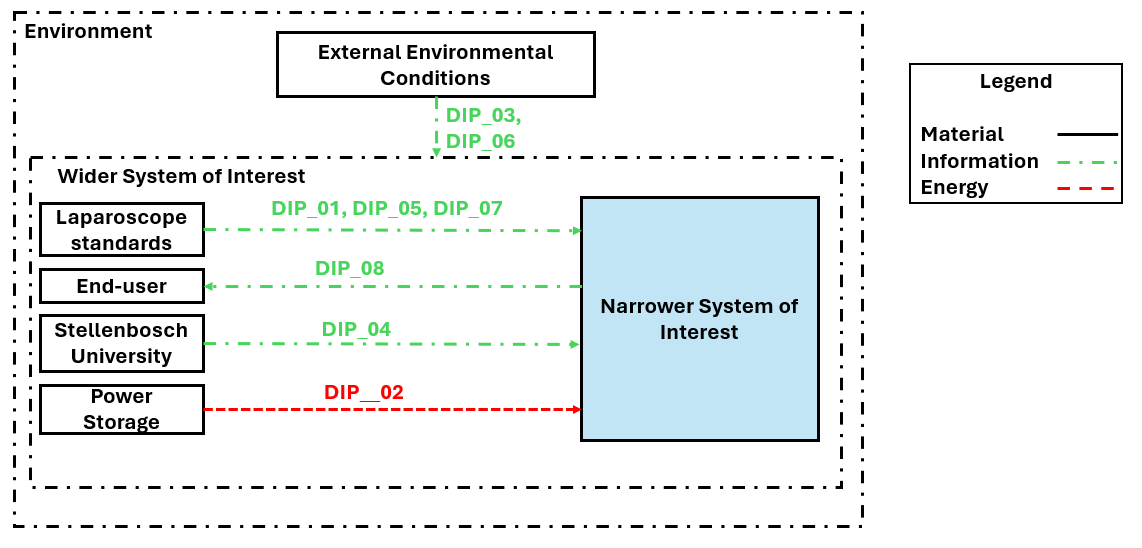
\includegraphics[height=6cm]{figs/System Boundary.png}
    \caption{System boundary}
    \label{fig:System Boundary}
\end{figure}



\subsection{Functional and Non-Functional Requirements}
Below in Table \ref{tab:FR} are the functional requirements for the laparoscope. Consequently, the Table \ref{tab:NFR} contains the non-functional requirements.

\begin{longtable}{|p{0.10\textwidth}|p{0.55\textwidth}|p{0.25\textwidth}|}


\caption{Functional requirements}
\label{tab:FR} \\

% ---- FIRST PAGE HEADER ----
\hline
\textbf{FR\_ID} & 
\textbf{Functional Requirement Description} & 
\textbf{Primary/Derived} \\
\hline
\endfirsthead

% ---- SUBSEQUENT PAGE HEADER ----
\hline
\textbf{FR\_ID} & 
\textbf{Functional Requirement Description} & 
\textbf{Primary/Derived} \\
\hline
\endhead

% ---- FOOTER ALL PAGES EXCEPT LAST ----
\hline
\multicolumn{3}{r|}{\textit{Continued on next page...}} \\
\hline
\endfoot

% ---- LAST PAGE FOOTER ----
\endlastfoot

% ---- DATA ROWS ----
FR\_1 & User interface & Primary \\
\hline

FR\_2 & System processor & Primary \\
\hline

FR\_3 & Power supply & Primary \\
\hline

FR\_4 & Operate Camera Module & Primary \\
\hline

FR\_4.1 & Specify camera settings & Derived \\
\hline

FR\_4.2 & Specify light intensity & Derived \\
\hline

FR\_4.3 & Capture digital image & Derived \\
\hline

FR\_5.0 & Display real-time images & Primary \\
\hline

FR\_6.0 & Store system data & Primary \\
\hline

\end{longtable}

\begin{longtable}{|p{0.12\textwidth}|p{0.25\textwidth}|p{0.55\textwidth}|}

\caption{Non-functional requirements}
\label{tab:NFR} \\

% ---- FIRST PAGE HEADER ----
\hline
\textbf{NFR\_ID} & 
\textbf{Non-Functional Requirement} & 
\textbf{Description}       \\                    
\hline
\endfirsthead

% ---- SUBSEQUENT PAGE HEADER ----
\hline
\textbf{NFR\_ID} & 
\textbf{Non-Functional Requirement} & 
\textbf{Description} \\                         % ← Please provide last column heading
\hline
\endhead

% ---- FOOTER ALL PAGES EXCEPT LAST ----
\hline
\multicolumn{3}{r|}{\textit{Continued on next page...}} \\
\hline
\endfoot

% ---- LAST PAGE FOOTER ----
\endlastfoot

% ---- NFR_01 ----
NFR\_01 & 
Relevant \mbox{compliance} & 
The design of the system should meet the relevant 
prescribed standard for this project, to ensure that 
the laparoscope meets all physical capabilities and 
functionality of a real laparoscope     \\                            
\hline

% ---- NFR_02 ----
NFR\_02 & 
Documentation & 
The design, implementation, construction, maintenance 
and testing procedures for the system should be 
thoroughly documented       \\                           
\hline

% ---- NFR_03 ----
NFR\_03 & 
Availability & 
The components for this project should be available 
to purchase if a component breaks or should be 
replaced \\
\hline

% ---- NFR_04 ----
NFR\_04 & 
Adjustable & 
The system design should be developed so that distinct 
features can be changed without creating large 
external costs \\
\hline

% ---- NFR_05 ----
NFR\_05 & 
Usability & 
The system should be easy to operate with limited training 
users \\
\hline

\end{longtable}


\subsection{Technical Performance Measures}


The technical performance measures (TPM) can be seen in the Table \ref{tab:FR-TPM} below, based on the requirements in Table \ref{tab:FR}. The reasoning behind all the TPM target values can be found below the table.

\begin{longtable}{|p{0.1\textwidth}|p{0.15\textwidth}|p{0.11\textwidth}|p{0.25\textwidth}|p{0.20\textwidth}|}

\caption{Technical performance measures}
\label{tab:FR-TPM} \\

% ---- FIRST PAGE HEADER ----
\hline
\textbf{FR\_ID} & 
\textbf{Function} & 
\textbf{TPM\_ID} & 
\textbf{TPM Description} & 
\textbf{TPM Target Value(s)} \\
\hline
\endfirsthead

% ---- SUBSEQUENT PAGE HEADER ----
\hline
\textbf{FR\_ID} & 
\textbf{Function} & 
\textbf{TPM\_ID} & 
\textbf{TPM Description} & 
\textbf{TPM Target Value(s)} \\
\hline
\endhead

% ---- FOOTER ALL PAGES EXCEPT LAST ----
\hline
\multicolumn{5}{r|}{\textit{Continued on next page...}} \\
\hline
\endfoot

% ---- LAST PAGE FOOTER ----
\endlastfoot

% ---- FR_1.0 - User Interface (2 TPMs) ----
\multirow{2}{*}{FR\_1.0} & 
\parbox[t]{\linewidth}{User \mbox{interface}} & 
TPM\_01 & 
Minimum user interface input(s) & 
$\geq$ 1 input \\
\cline{3-5}

& & 
TPM\_02 & 
Minimum user interface signal(s) & 
$\geq$ 1 signal light \\
\hline

% ---- FR_2.0 - System Processor (1 TPM) ----
FR\_2.0 & 
System \mbox{processor} & 
TPM\_03 & 
Minimum GPIO pins & 
$\geq$ 1 GPIO Pin \\
\hline

% ---- FR_3.0 - Power Supply (2 TPMs) ----
\multirow{2}{*}{FR\_3.0} & 
\parbox[t]{\linewidth}{Power \mbox{supply}} & 
TPM\_04 & 
System start-up cycle duration & 
$\leq$ 2 s \\
\cline{3-5}

& & 
TPM\_05 & 
Total duration of power supply required & 
$\geq$ 6.7 hours \\
\hline

% ---- FR_4.0 - Operate Camera Module (3 TPMs) ----
\multirow{3}{*}{FR\_4.0} & 
\parbox[t]{\linewidth}{Operate camera module} & 
TPM\_06 & 
Amount of camera modules & 
1 camera modules \\
\cline{3-5}

& & 
TPM\_07 & 
Working length of the system & 
300 mm \\
\cline{3-5}

& & 
TPM\_08 & 
Viewing angle of camera module & 
30$^{\circ}$ \\
\hline

% ---- FR_4.1 - Configure Camera Properties (1 TPM) ----
FR\_4.1 & 
\makecell[l]{Configure \\camera \\properties} & 
TPM\_09 & 
Focus depth of the camera module & 
30 mm - 80 mm \\
\hline

% ---- FR_4.2 - Configure Light Intensity (2 TPMs) ----
\multirow{2}{*}{FR\_4.2} & 
\parbox[t]{\linewidth}{Configure light \mbox{intensity}} & 
TPM\_10 & 
Illumination of the system & 
40 000 LUX - 160 000 LUX \\
\cline{3-5}

& & 
TPM\_11 & 
Maximum surface temperature & 
$\leq$ 41 $^{\circ}$C \\
\hline

% ---- FR_4.3 - Capture Digital Image (2 TPMs) ----
\multirow{3}{*}{FR\_4.3} & 
\parbox[t]{\linewidth}{Capture digital image} & 
TPM\_12 & 
Minimum field of view & 
$\geq$ 70$^{\circ}$ \\
\cline{3-5}

& & 
TPM\_13 & 
Minimum resolution & 
460 x 460 pixels \\
\cline{3-5}

& & 
TPM\_14 & 
Minimum frame rate & 
10 fps \\
\hline

% ---- FR_5.0 - Display Real-Time Images (2 TPMs) ----
\multirow{2}{*}{FR\_5.0} & 
\parbox[t]{\linewidth}{Display real-time images} & 
TPM\_15 & 
Minimum resolution of display & 
460 x 460 pixels \\
\cline{3-5}

& & 
TPM\_16 & 
Maximum latency & 
0.5 s \\
\hline

% ---- FR_6.0 - Store System Data (1 TPM) ----
FR\_6.0 & 
Store system data & 
TPM\_17 & 
Storage capacity & 
68.56 GB \\
\hline

\end{longtable}

\begin{itemize}
     

    \item\textbf{TPM\_01:} The bare minimum for the laparoscope to function properly with user inputs is to at least install an on or off switch. It is the bare minimum required for this project.

    \item\textbf{TPM\_02:} For the operator to know the laparoscope is still functioning properly, without looking at the display screen or light module at the end of the laparoscope, there should be at least 1 signal light on the laparoscope to indicate that the system is receiving power.

    \item\textbf{TPM\_03:} To operate the signal lights the microcontroller or SBC will require GPIO pin to push current into the signal lights. Thus, the minimum required is the minimum of the laparoscope signal lights.

    \item\textbf{TPM\_04:} This is dependent on the component selected and the different interfaces selected between the different components. However, the desired start-up cycle duration should be less than two seconds.

    \item\textbf{TPM\_05:} The system should be able to power on for long durations of times. The total amount of time it should be powered on is the duration of a typical laparoscopic surgery. 

    \item\textbf{TPM\_06:} The system requires at least one laparoscopic camera. A second camera module can help the system achieve 3D visualization. Any additional cameras would be redundant for this project.

    \item\textbf{TPM\_07:} The system design should be similar to current laparoscopes. Current laparoscope designs has a working distance of 300 mm. The working distance is the distance of the rod that can be inserted into the patient's body.

    \item\textbf{TPM\_08:} Different laparoscope products have different viewing angles. Some has a viewing angle of 0°, while there are products that have a viewing angle of 90°. However, a common viewing angle is 30°, which is the value that will be pursued in this project.

    \item\textbf{TPM\_09:} The distance between the camera sensor of the laparoscope and the object that is being captured is the focus depth. 

    \item\textbf{TPM\_10:} The total illumination required per medical theatres.
    
    \item\textbf{TPM\_11:} The maximum temperature of the casing of the laparoscope tip, based on medical standards.

    \item\textbf{TPM\_12:} Smallest viewing angle applied to a laparoscopic commercial product is 70°,  while certain laparoscopes has a viewing angle larger than 70°.

    \item\textbf{TPM\_13:} The minimum resolution for the camera module is determined by first determining the maximum visible distance seen at the smallest fov, and multiplying that value by how many pixels a millimetre area should represent: 
    \begin{equation}
        Pixel = Focus depth_(max)*sin(fov/2)*2*5 pixels/mm
    \end{equation}

    \item\textbf{TPM\_14:} The maximum allowable time between frame is 0.1 S. Therefore, the minimum frame rate of the camera module is 10 fps.

    \item\textbf{TPM\_15:} The minimum resolution of the display is the same as the minimum resolution of the camera.

    \item\textbf{TPM\_16:} This value is subject to change based on the different components used for the system. Therefore, it is important to minimize the latency of each component or interaction between different components. 0.5 s is just an absolute maximum latency that will be accepted.

    \item\textbf{TPM\_17:} If the minimum resolution of an image is 460 x 460 with RGB colour format, then 1 image requires 634.8 KB. (PxP*24/8) If the frame rate is 30 fps and this continued for 60 minutes, then a total space of 68.5584 Gb is required.

\end{itemize}

\section{Concept Generation}

For this project, three concepts were generated, based on the principle that the design utilizes the DF Robot endoscope, which has the dimensions of Ø8~mm and a total length of 25~mm. This module was chosen since it is the maximum space required to fit all the necessary PCB and camera assembly to create an endoscope, which still fits within the Ø10~mm hole. Each concept is designed to have a viewing angle of 30°.

The first concept relies on bending the shaft that the endoscope camera is attached to. However, the total diameter of the laparoscope within the skin and muscle tissue of the patient should remain under the Ø10~mm limit since the thickness of the muscle and tissue of patients is not all the same; the design has to be made for the worst case scenario, which is for an obese patient around 10~cm. Figure \ref{fig:Concept 1} below illustrates how the design would look:

\begin{figure}[H]
    \centering
    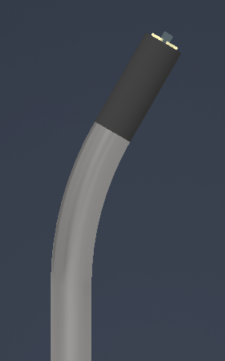
\includegraphics[height = 8 cm]{figs/Concept 1.png}
    \caption{Concept 1: Bent shaft design}
    \label{fig:Concept 1}
\end{figure}

The second concept relies on the fact that the lens assembly is tilted to 30° relative to the axial axis of the laparoscope. This concept does require careful hardware consideration and positioning; however is a proven method in the industry. Figure \ref{fig:Concept 2} illustrates this design:

\begin{figure}[H]
    \centering
    
\includegraphics[height = 8 cm]{figs/Concept 2.png}
    \caption{Concept 2: Tilted lens design}
    \label{fig:Concept 2}
\end{figure}

The last concept relies on a pulley system, which allows the camera to be tilted at a desired angle by the practitioner while the operation is being performed. This method relies on fine detail design, but can prove to be beneficial for future research purposes. The final concept is illustrated in Figure \ref{fig:Concept 3} below:

\begin{figure} [H]
    \centering
    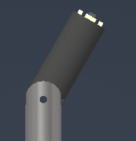
\includegraphics[height = 8 cm]{figs/Concept 3.png}
    \caption{Concept 3: Adjustable viewing angle design}
    \label{fig:Concept 3}
\end{figure}

All three concepts mentioned above can be used for the project, since they meet all the physical demands of the laparoscope. However, each concept has its defects. Concepts one and three both have a defect when their camera is tilted at 30°. When the laparoscope is being rotated, there might be vital information that is missed in the direction of the laparoscope's axial axis, due to the camera lenses not being centred on the axis itself. It can also possibly cause damage to the patients if the laparoscopes are turned and accidentally pushed into the patient's internal organs.

Due to the reason stated above, the second concept is the preferred concept that will be further developed.

\section{Detailed Drawing}

Based on the previous section, it was determined to use the tilted camera design. A common problem with laparoscopes and endoscopes is the small scale of the design. There are limited commercial products for such a small-scale design. Consequently, it leads to the design and manufacturing of custom parts that can perform the required duties, with size constraints. This design, however, adds additional complexity with the camera module and light source of the laparoscope being mounted to the tip of the laparoscope. These two components generate heat, which should not be transferred into the "patient's" body. Therefore, the design should account for this by minimizing the total heat transferred into the "patient's" body or by maximizing the total heat transferred through the laparoscope outside the "patient's" body.

This design also reduces the complexity of the design due to the placements of the camera module and light source. For a conventional laparoscope, either the camera module or the light source or both, are placed outside the patients body. This design requires the complex lens assemblies for the camera module to be able to view inside the "patient's" body, with the addition of plastic optical fiber cables for the light source.

To design for the heat problem, there are two main methods to control the heat dissipation of the camera module and light source:

\begin{itemize}
    \item Actively cool down the heat sources while they are being operated.
    \item Actively conduct the heat from the heat source, located at the tip, to the base of the laparoscope, where the heat can be more easily dissipated.
\end{itemize}

The first method, however functional, is not a practical solution for this design, due to the size constraints. For this method to work, cold air should be blown to the tip of the laparoscope, while warm air should also be extracted from the tip. Therefore, 2 ventilation tubes should lead down from the handle of the laparoscope to the tip of the laparoscope, while being confined in a Ø~8~mm hole. Additionally, it should provide space for the wiring of the camera module and heat sources.  It is important that air should both be extracted and provided to the tip of the laparoscope, from the handle, and cannot be extracted from or dispersed into the "patient's" body. Otherwise, this design will not function as a medical laparoscope. Due to the limitations stated above, this design is not feasible.

The second method, however, has been accomplished. A patent has been filed with the United States Patent and Trademark Office (USPTO), which utilizes heat pipes to conduct the heat from the light source at the tip of the laparoscope to a heat sink in the handle of the laparoscope. \citep{USP-1} However, this patent is only designed to conduct heat generate by the light source, while the design that will be pursued will also account for the laparoscope camera module heat generation. 

A critical feature of this design is the physical hardware. Heat pipes and heat sinks are required to sufficiently conduct the heat as well as properly dissipate the conducted heat safely and efficiently out of the product. Fortunately, RS Components provides both heat pipes and heat sinks in a wide variety of sizes. Importantly, the smallest diameter heat pipes they sell are 3~mm, at a maximum length of 250~mm. However, TPM\_07 dictates that the working length of the laparoscope should be 300~mm. Therefore, a combination of heat pipes will be required to conduct the generated heat from the tip all the way to the heat sinks, through means of a coupler. \citep{RS}

Another coupler is required to attach at the tip of the furthest heat pipe from the handle, to be able to conduct the generated heat from the camera module and light source properly to the heat pipes. However, this coupler will require additional modification to account for the PCB of the camera module and light source. It requires a design balance to ensure that there is enough material to properly conduct the heat to the heat pipes, while allowing the camera module and light source to operate properly and is not constricted by the design. 

A Stainless steel pipe will be utilized to act as a cover for the entire laparoscope's working length, keeping everything together and protected. Stainless steel was selected due to its being the only commercial material that is produced with such small dimensions. 

For the handle of the laparoscope, 3D printing was selected to create a custom handle for the laparoscope, due to its ability to create custom components. However, an important decision was made to use acrylonitrile butadiene styrene (ABS) filament instead of polylactic acid (PLA) filament. ABS filament, although harder to print, has higher temperature tolerances and can withstand mechanical loads better. 

Figure \ref{fig:Full Assembly} below shows the full assembly of the laparoscope, while Figure \ref{fig:Main Assembly}, shows the assembly of the main body of the laparoscope. The full assemblies of these design can be seen in the Appendix \ref{sec:Drawings}, with the drawing tree as well.

\begin{figure}[H]
    \centering
    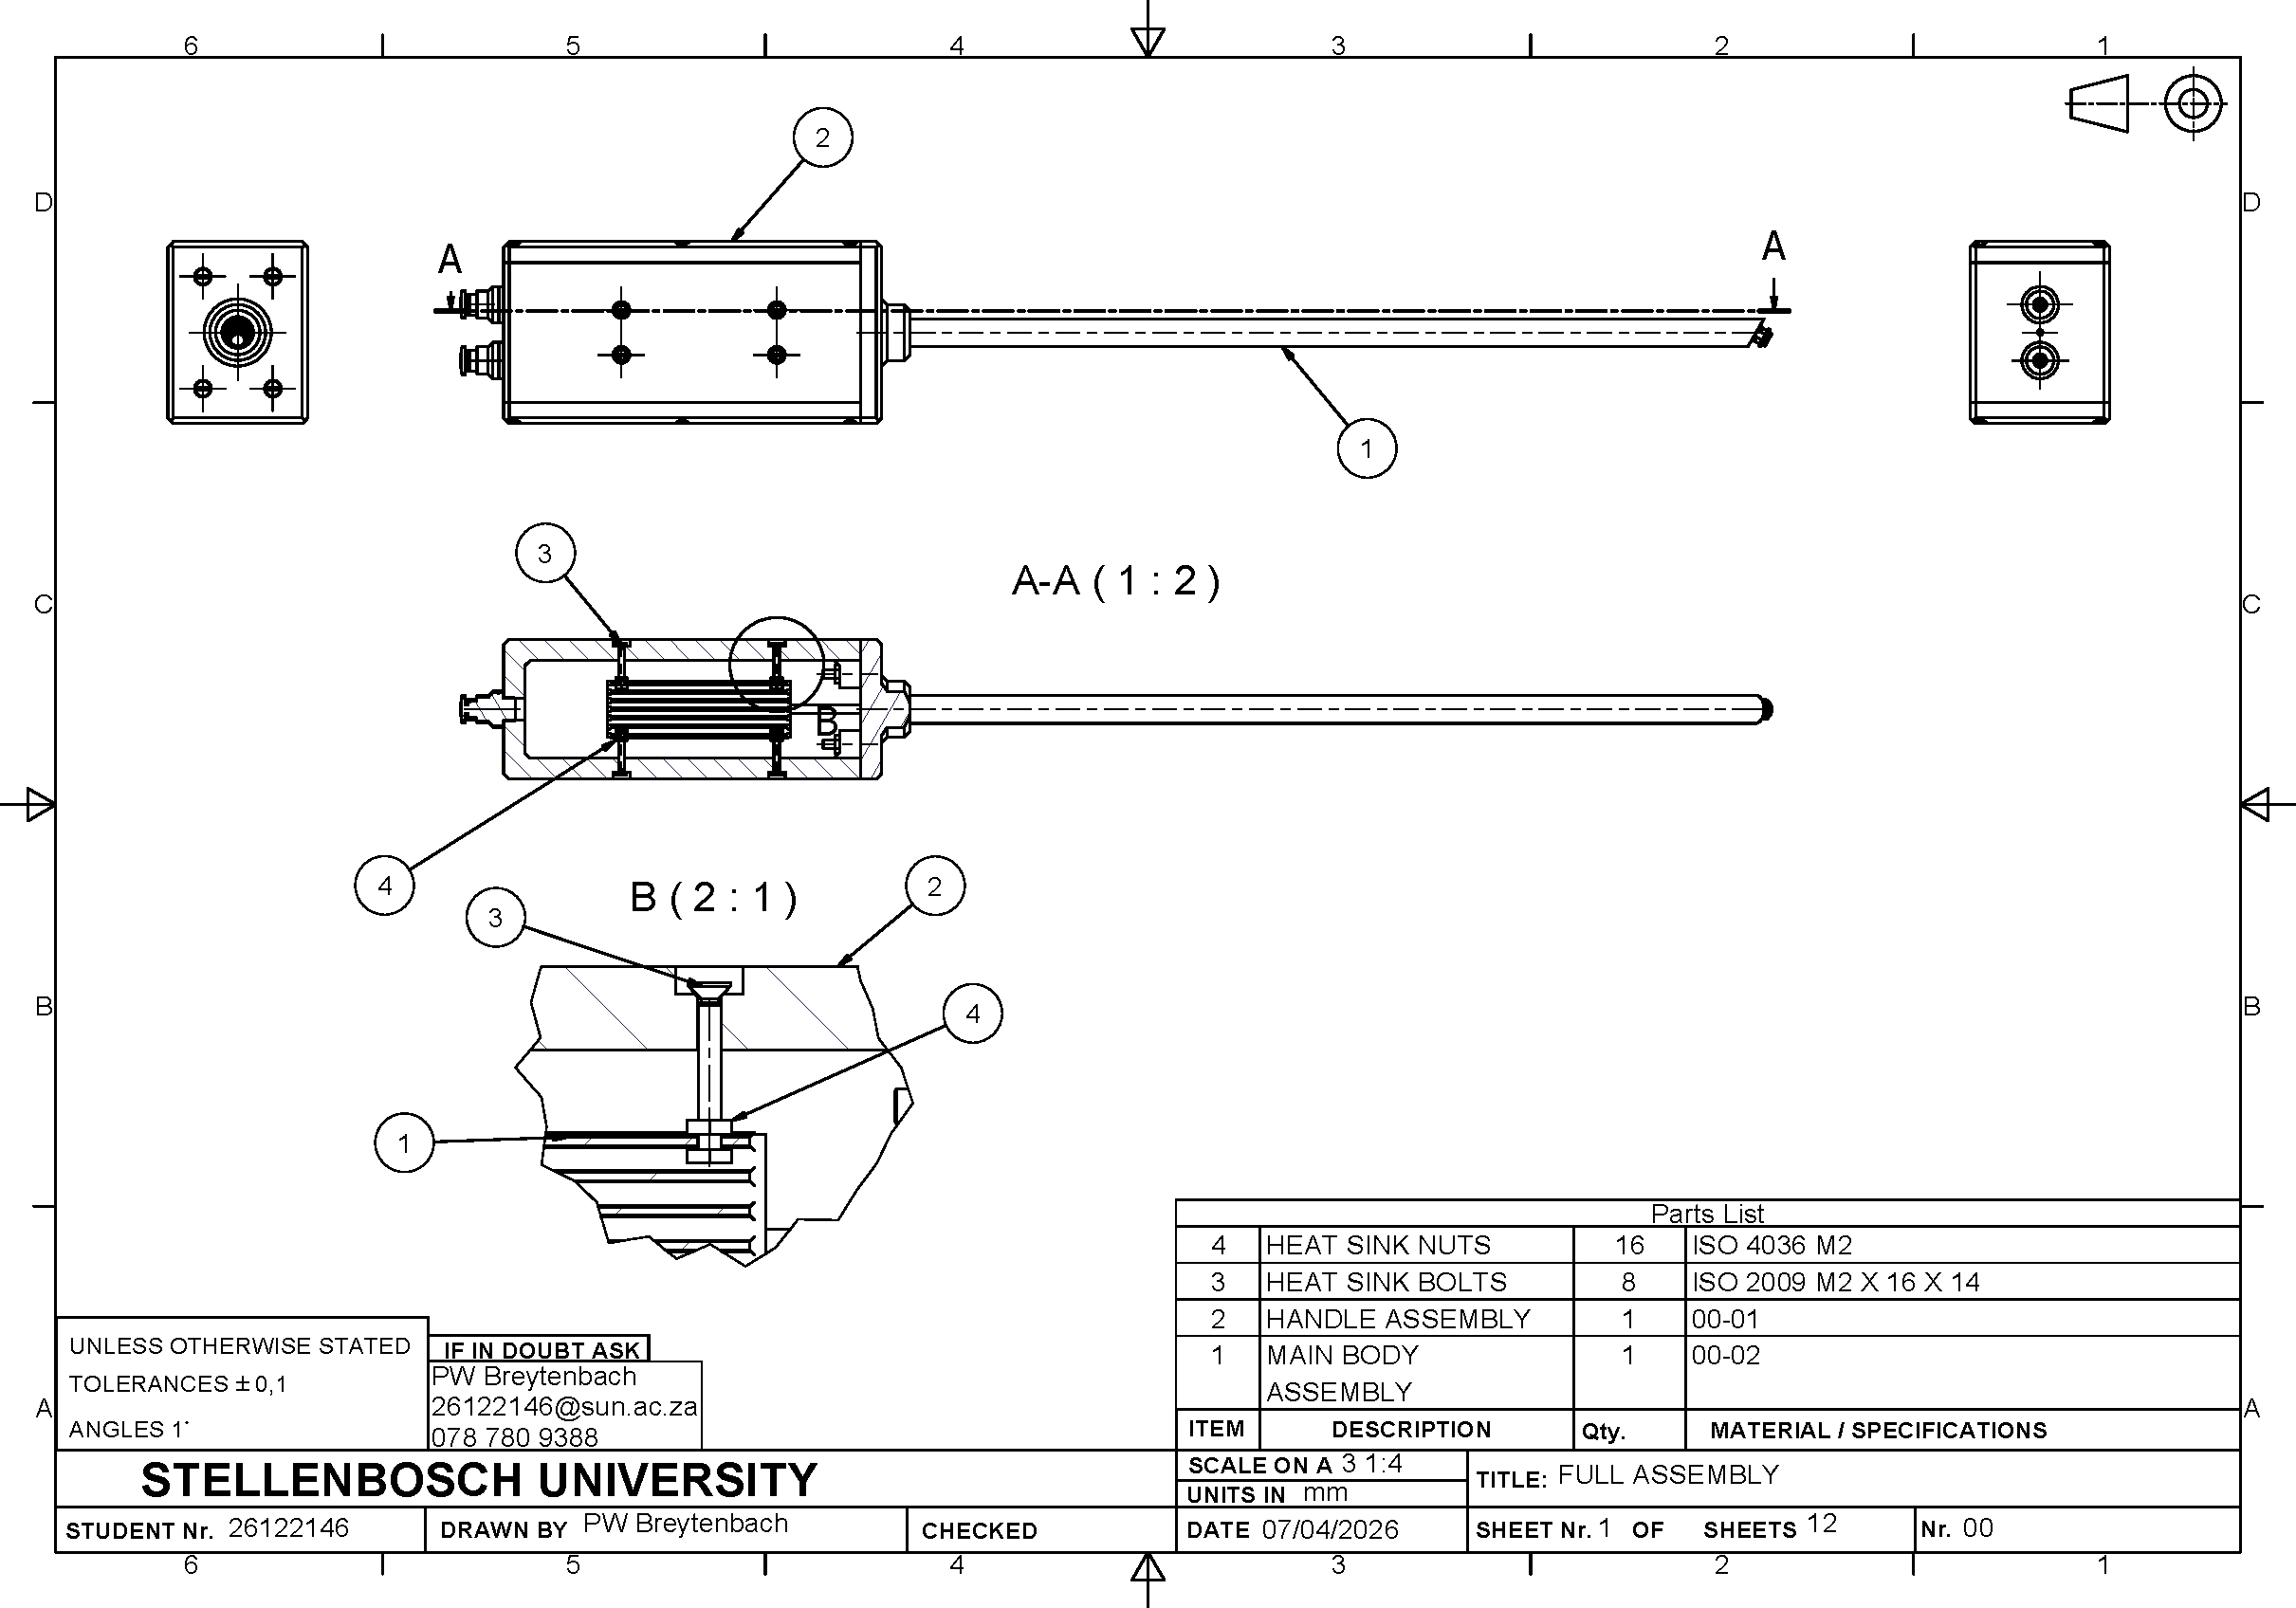
\includegraphics[width=\linewidth, keepaspectratio]{PDFs/FULL_ASSEMBLY.pdf}
    \caption{Full assembly drawing}
    \label{fig:Full Assembly}
\end{figure}

\begin{figure}[H]
    \centering
    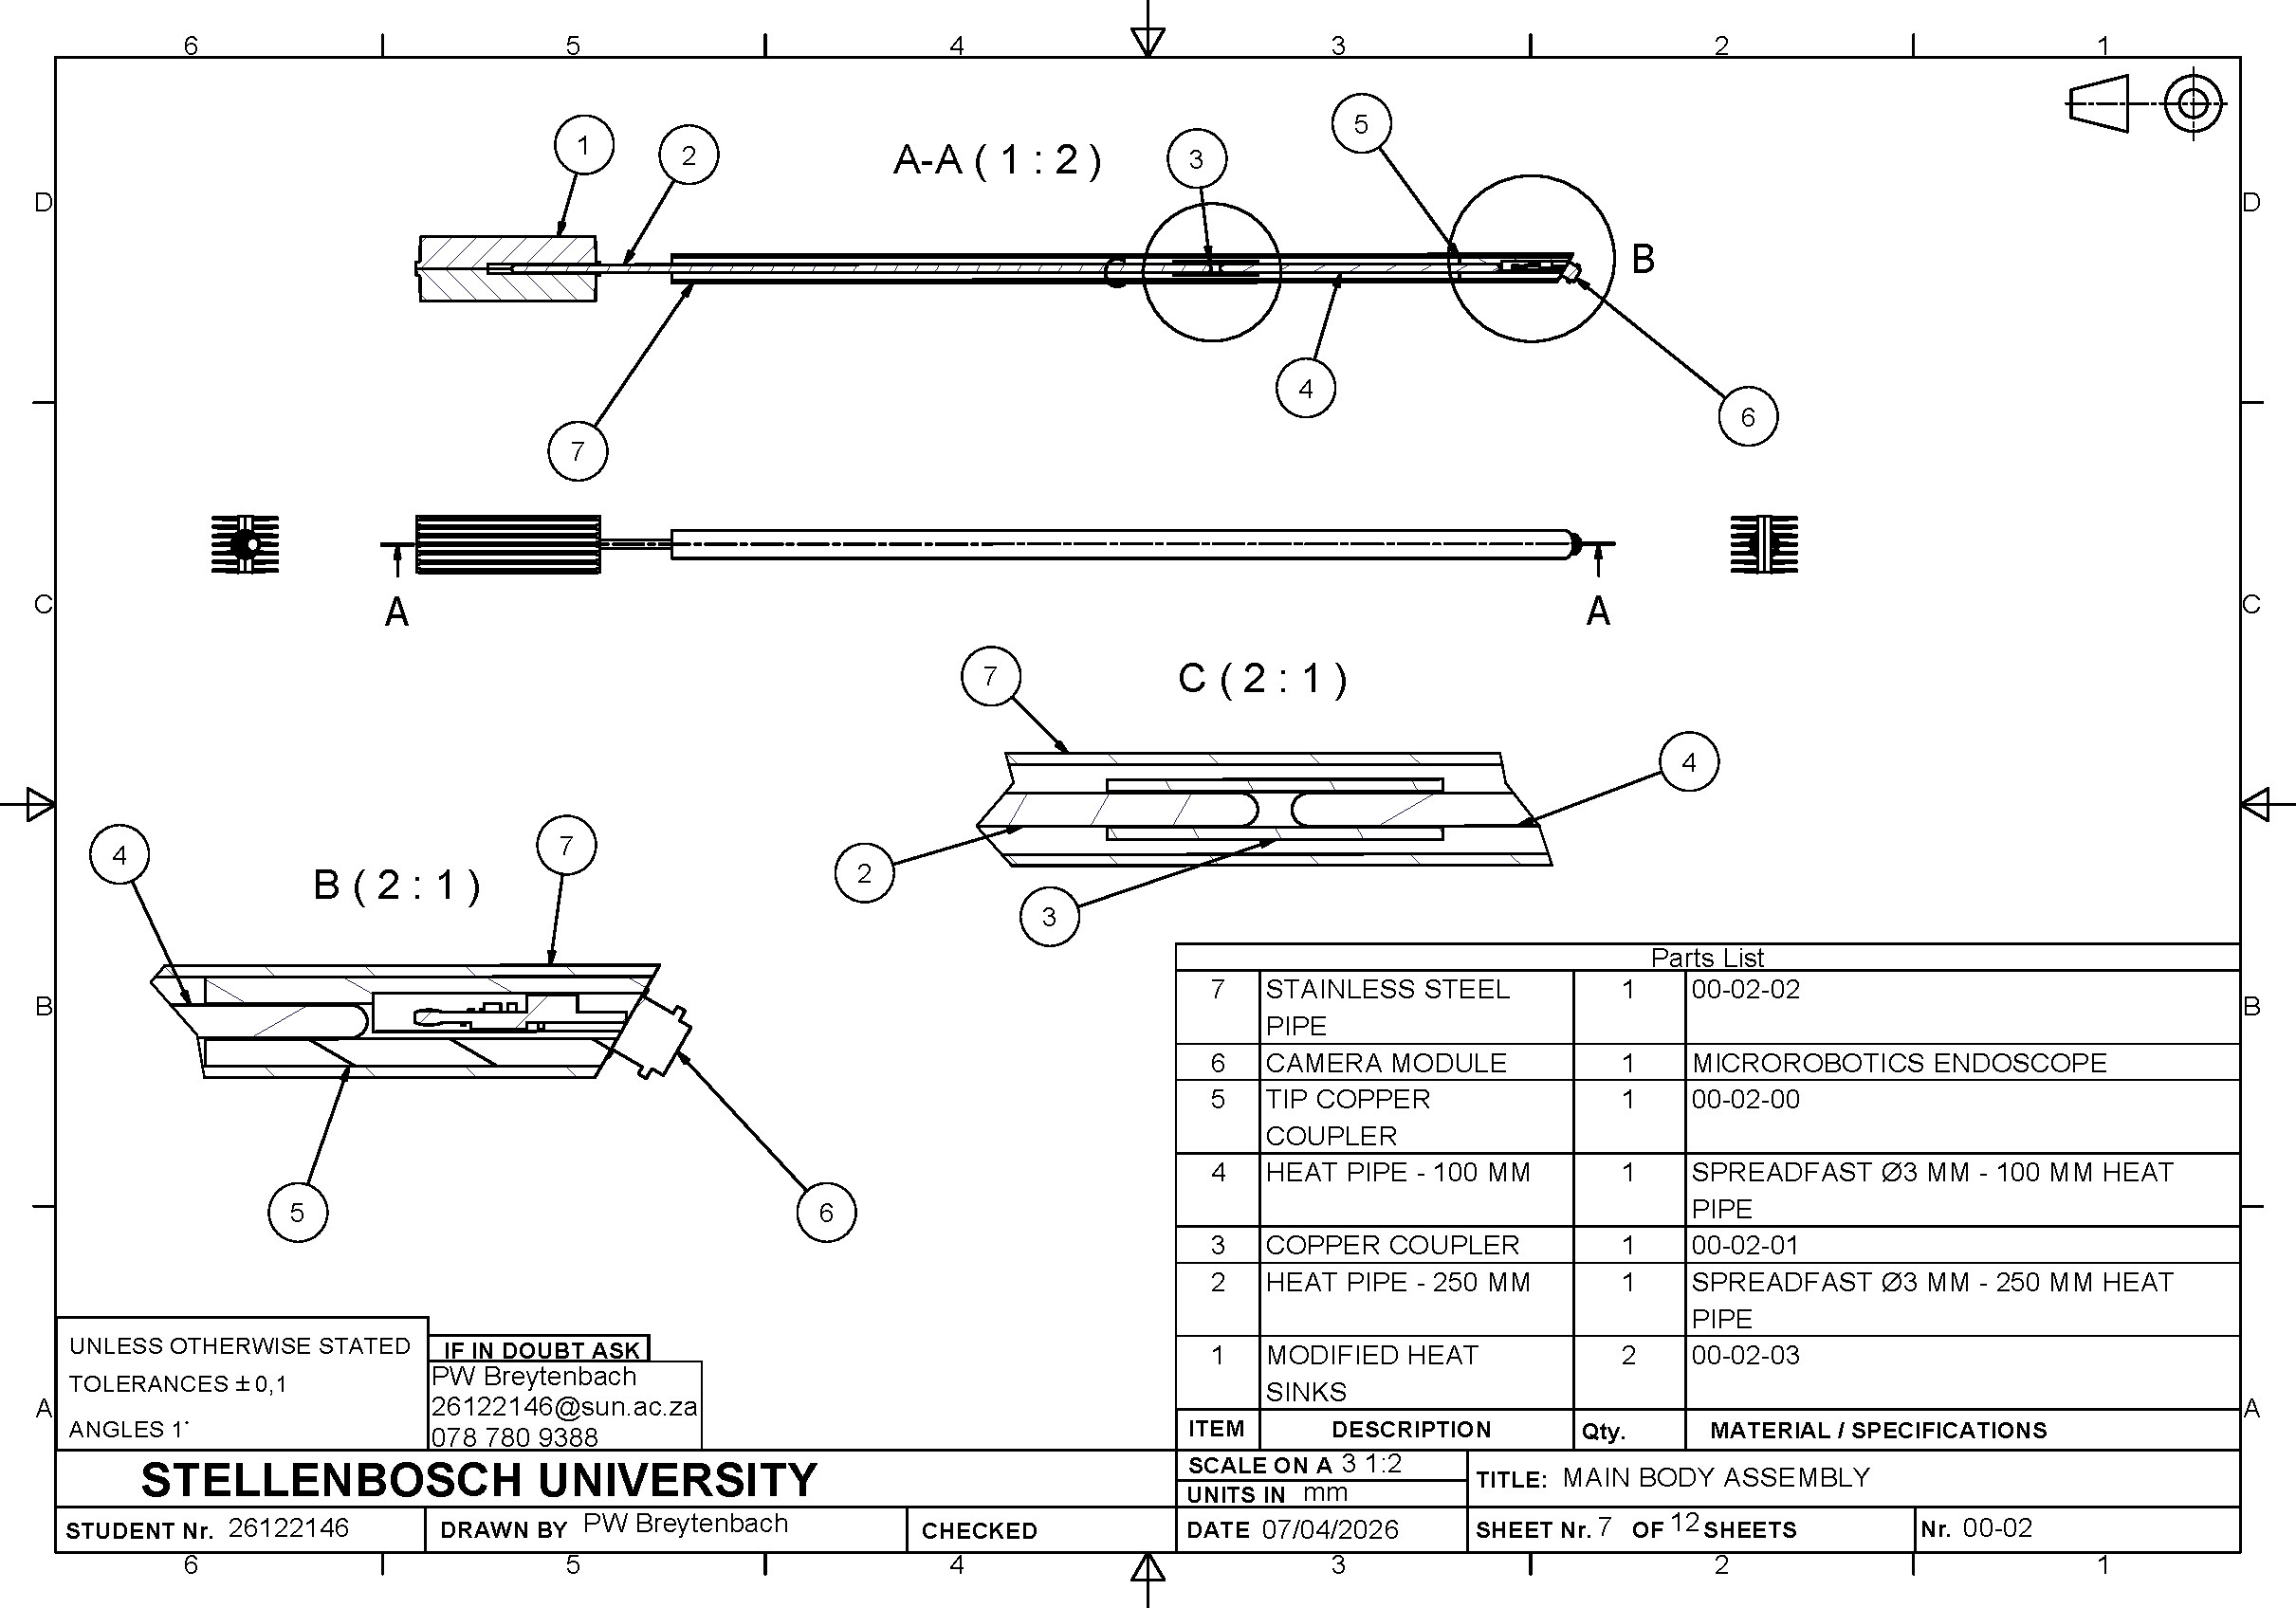
\includegraphics[width=\linewidth, keepaspectratio]{PDFs/Main_Body_Assembly.pdf}
    \caption{Main body assembly drawing}
    \label{fig:Main Assembly}
\end{figure}


